\documentclass[11pt,a4paper]{article}
\usepackage[german]{babel}
\usepackage[utf8]{inputenc}
\usepackage[T1]{fontenc}
\usepackage{amsmath,amssymb,amsfonts}
\usepackage{graphicx}
\usepackage{fancybox}

% Blackboard bold symbols (formerly from mathsym.sty at IAKS Karlsruhe)
\newcommand{\R}{{\mathbb{R}}}
\newcommand{\C}{{\mathbb{C}}}

\newcommand{\betrag}[1]{|#1|}
\newcommand{\fourier}[1]{\mathcal{F}\left( #1\right)}
\newcommand{\norm}[1]{\parallel #1 \parallel_{W_{Signal}}}
\newcommand{\snr}[2]{\mbox{SNR}_I ( #1, #2 )}
\newcommand{\skalar}[2]{\left< #1, #2 \right>_{W_{Signal}}}

\pagestyle{empty}
\advance\rightmargin22mm
\begin{document}
{\Large
\begin{center}
%%\vspace*{1cm}
{\huge\bf Entwurf diffraktiver Strahlformer mit der Methode der finiten Elemente} \\[1cm]
\begin{figure}[htb]
   \centerline{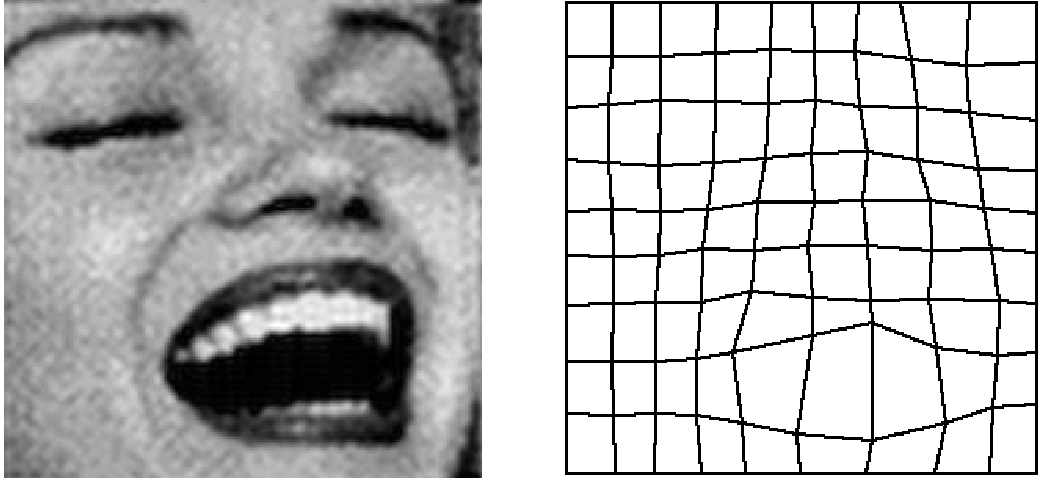
\includegraphics[width=6cm]{titelbild}}
\end{figure}
{\em Eine Studienarbeit von}\\[1cm]
{\LARGE\bf Pawel Wocjan}\\[1cm]
{\em am}\\[1cm]
{\LARGE Institut f"ur Algorithmen und Kognitive Systeme}\\
{\LARGE Fakult"at f"ur Informatik, Universit"at Karlsruhe (TH)}\\[1cm]
{\em unter Betreuung von}\\[1cm]
{\LARGE Prof.~Dr.~Th.~Beth}\\
{\LARGE Dipl.--Inform.~M.~Schmid}\\
\vfill

Sommersemester 1997\\
\vfill
\end{center}
}

\LARGE

\setlength{\parindent}{0mm}

\newpage
  \begin{center}
    {\huge\bf Diffraktive Optik - kurze Einf"uhrung des Modells }
  \end{center}
  \vfill
  \begin{itemize}
    \item Es wird die {\em skalare Beugungstheorie} benutzt.   
      \vfill
    \item {\em Wellenfronten} werden durch zweidimensionale Signale beschrieben
       $$ f : \left\{
                 \begin{array}{rcl}
                  \R^2  & \longrightarrow & \C \\
                  (x,y) & \longmapsto     & A(x,y) \exp (i\phi (x,y)).
                 \end{array}
               \right.
       $$ 
      \vfill
    \item {\em Diffraktive Elemente (DE)} werden durch \\ {\em Transmissionsfunktionen}
       $T_{DE}$ beschrieben
       $$ T_{DE} : \left\{
                      \begin{array}{rcl}
                        \R^2  & \longrightarrow & \C \\
                        (x,y) & \longmapsto     & A(x,y) \exp (i\phi (x,y)).
                      \end{array}
                    \right.
       $$ 
  \end{itemize}

\newpage
  \begin{center}
    {\huge\bf Einf"uhrung des Modells}
  \end{center}
  \vfill
  \begin{figure}[htb]
    \centerline{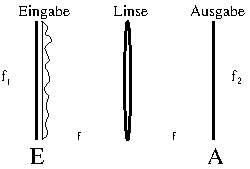
\includegraphics[width=8cm]{aufbau}}
  \end{figure}
  \vfill
  \begin{itemize}
    \item Die Wirkung eines DEs auf eine Wellenfront entspricht der
       punktweisen Multiplikation des Signals mit der Transmissionsfunktion.
      \vfill
    \item Die 2D-Fourier-Transformation $\mathcal{F}$
      beschreibt die Wellenausbreitung von $E$ nach $A$.
  \end{itemize}
  \vfill
  \begin{center} 
    {\bf Zentrales Problem}
  \end{center}
  \vfill
    Berechne eine Transmissionsfunktion $T_{DE}$ mit 
    $$\mathcal{F}(T_{DE} f_1) = f_2, $$
    wobei $T_{DE}\in\mathcal{D}$, d.h. gewissen Einschr"ankungen unterliegt
    (z.B. $\betrag{T_{DE}(x,y)} = 1$).
  \vfill

\newpage
  \begin{center}
    {\huge\bf Die Methode der station"aren Phase}
  \end{center}
  \vfill
   \begin{figure}[htb]
     \centerline{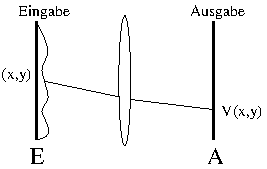
\includegraphics[width=8cm]{stat}}
  \end{figure}
  \vfill
  Das diffraktive Phasenelement (DPE) realisiert \\
  eine Verzerrung $V$, wenn
  $$ \nabla\phi(x,y) = \frac{2\pi}{\lambda f} V(x,y) $$
  gilt. Die Verzerrung mu"s glatt sein.
  \vfill
 \newpage
  \begin{center}
    {\huge\bf Analytische Methode}
  \end{center}  
  \vfill
  In vielen F"allen ist nur die Intensit"at wichtig.
  \vfill
  \begin{itemize}
    \item Finde eine Verzerrung $V$, die die Intensit"at von $f_1$ in
      die Intensit"at von $f_2$ umverteilt.
    \item Berechne das DPE mit der Methode der station"aren
      Phase.
  \end{itemize}
  \vfill
  \begin{figure}[htb]
    \centerline{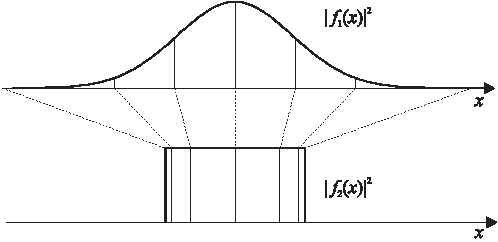
\includegraphics[width=7cm]{distort}}
  \end{figure}
  \vfill
  Verzerrung $V$ einfach zu berechnen, wenn
  $f_1$ und $f_2$ beide 
  \begin{itemize}
    \item {\bf separabel} oder
    \item {\bf isotrop}
  \end{itemize}
  sind.
  \vfill  
  F"ur viele Signale ist es nicht m"oglich, so eine Verzerrung $V$ zu finden
  (wenn Cauchy-Riemannsche-Bedingung nicht erf"ullt).
  
\newpage
  \begin{center}
    {\huge\bf 2. Bestimmung der Phasenfunktion mit den generierten Netzen}
  \end{center}
  \vfill
  Die Phasenfunktion $\phi(x,y)$ wird durch ein bivariates Polynom vom 
  Grad $D-1$ angen"ahrt.
  $$ \phi(x,y) = \sum_{k=0}^{D-1}\sum_{l=0}^{D-1-k} a_{kl}\cdot x^k y^k, $$    
  \vfill
  Nach der Methode der station"aren Phase mu"s gelten:
  $$ \nabla \phi(x_{ij},y_{ij}) = T(x_{ij},y_{ij}) = \begin{pmatrix} \phi_x^{ij} \\ \phi_y^{ij}\end{pmatrix}. $$
  \vfill
  Bestimme die $a_{kl}$ mit der
  Methode der kleinsten Quadrate.  Das f"uhrt auf ein LGS f"ur die Unbekannten $a_{kl}$.
  \vfill

\newpage
  \begin{center}
    {\huge\bf Vergleich mit anderen Methoden}
  \end{center}
  \vfill
  Eingabesignal: $f_1$

  Ausgabesignal: $f_2$

  das realisierte Signal: $ f(x)=\mathcal{F}\left\{f_1 T_{DPE}\right\}(x) $
  \vfill
  {\bf Das Signal-Rausch-Verh"altnis:}
  $$ \snr{f_2}{f} = \frac{\norm{f}^2} {\norm{\betrag{f_2}-\alpha\betrag{f}}^2} $$
  mit dem Skalierungsfaktor
  $$ \alpha = \frac{\skalar{\betrag{f}}{\betrag{f_2}}}{\norm{f}^2}. $$
  \vfill
  {\bf Die Beugungseffizienz $\eta$}
  $$ \eta = \frac{\norm{f}}{\parallel f_1 \parallel_{W_{DE}}^2} $$
  \vfill

\newpage
  \begin{center}
    {\huge\bf Schlu"sbetrachtung}
  \end{center}
  \vfill
  \begin{itemize}
    \item Die Methode der finiten Elemente ist eine neue Methode, gute Startwerte f"ur 
      IFTA zu berechnen.
      \vfill
    \item Sehr gro"se Beispiele k"onnen speichereffizient berechnet werden.
      \vfill
    \item Ein gro"ser Nachteil besteht darin, da"s viele Parameter richtig gew"ahlt werden
      m"ussen.
      \vfill
    \item Je gr"o"ser die Knotenanzahl $s$ verwendet werden, desto besser das Ergebnis.
      \vfill
    \item Der Grad $D$ sollte kleiner sein als die H"alfte der Knotenanzahl $s$
      gew"ahlt werden, weil sonst "Uberschwinger bei der Approximation entstehen.
   \end{itemize}
   \vfill
\end{document}


